% =====================================================================
% ejercicio08.tex
% Responsabilidad única: ajustar la regresión logística regularizada en el caso cáncer de mama,
% seleccionar $C$ por ROC-AUC de validación y fijar el umbral por costo.
% Las cifras provienen de generado/resultados.tex y generado/tabla_*.tex.
% =====================================================================
\subsection{Ejercicio 8: Caso B, regresión logística y elección del umbral}

\paragraph{Qué buscamos.} Pasamos al caso del cáncer de mama, donde hay
que decidir si una muestra es maligna. Usamos la regresión logística de
los ejercicios 3 y 4, ahora con los $30$ predictores estandarizados. Hay
dos decisiones que tomar con validación y en este orden: primero cuánto
regularizar (el hiperparámetro $C$), lo que fija el modelo y sus
probabilidades, y después a partir de qué probabilidad declaramos una
muestra como maligna (el umbral $t$), lo que convierte probabilidades en
decisiones.

\begin{enumerate}

\item \textbf{Particiones, recodificación y referencia.}
Antes de ajustar nada quisimos estar seguros de la recodificación, así que
hicimos una tabla cruzada (un conteo de cuántas muestras hay en cada
combinación de etiqueta original y etiqueta nueva): los 212 tumores
\texttt{malignant} quedaron con $y=1$ y los 357 \texttt{benign} con
$y=0$, de modo que las métricas de la clase positiva hablan de muestras
malignas. La proporción de malignos fue $\PropMalTr$ en entrenamiento y
$\PropMalVal$ en validación, prácticamente iguales gracias a la
estratificación.

Como referencia usamos \texttt{DummyClassifier} con
\texttt{strategy="prior"}, que le asigna a todas las muestras la misma
probabilidad de maligno, la proporción de entrenamiento ($\PropMalTr$).
Como esa probabilidad es menor que $0.5$, con $t=0.5$ predice siempre
benigno: no tiene verdaderos ni falsos positivos. Su precisión,
$TP/(TP+FP)=0/0$, queda indefinida, y el argumento \texttt{zero\_division=0}
le dice a scikit-learn que la reporte como 0, al igual que el recall
($0$ malignos detectados) y el F1. Su ROC-AUC es exactamente $0.5$: como da
el mismo puntaje a todas las muestras, no pone ningún maligno por encima
de ningún benigno, y eso es lo mismo que ordenar al azar.

\item \textbf{Selección de $C$.}
Probamos $C\in\{0.01,\,0.1,\,1,\,10\}$, de mucha a poca regularización
(recordemos del Ejercicio~4e que un $C$ pequeño castiga más los
coeficientes). Como criterio usamos el ROC-AUC de validación porque no
depende del umbral, que todavía no habíamos elegido: mide qué tan bien el
modelo \emph{ordena} las muestras, poniendo las malignas por encima de las
benignas.

\begin{table}[H]
\centering
\resizebox{\textwidth}{!}{% Archivo generado automáticamente por el notebook (no editar a mano).
\begin{tabular}{lrrrrrl}
\toprule
C & ROC-AUC ent. & ROC-AUC val. & F1 ent. (t=0.5) & F1 val. (t=0.5) & Iteraciones & Convergió \\
\midrule
0.01 & 0.9927 & 0.9905 & 0.9283 & 0.9512 & 10 & Sí \\
0.1 & 0.9955 & 0.9951 & 0.9721 & 0.9762 & 10 & Sí \\
1 & 0.9979 & 0.9957 & 0.9840 & 0.9655 & 18 & Sí \\
10 & 0.9997 & 0.9957 & 0.9960 & 0.9545 & 33 & Sí \\
\bottomrule
\end{tabular}
}
\caption{Regresión logística según $C$: ROC-AUC y F1 ($t=0.5$) en entrenamiento y validación, y convergencia.}
\label{tab:ex8-C}
\end{table}

El ajuste usa el algoritmo \texttt{lbfgs}, que, como el descenso de
gradiente del Ejercicio~4c, mejora los coeficientes paso a paso hasta que
los cambios son despreciables. Decimos que \emph{convergió} si llegó a ese
punto antes del límite de pasos que le fijamos. Los cuatro ajustes
convergieron (como máximo $\LogitIterMax$ iteraciones, lejos del límite de
5000, y sin la advertencia \texttt{ConvergenceWarning}).

El ROC-AUC de validación creció con $C$ hasta estabilizarse
(Tabla~\ref{tab:ex8-C}), y nos encontramos con que $\LogitEmpatesC$
valores de $C$ ($C=1$ y $C=10$) obtuvieron exactamente el mismo máximo a
precisión completa (que redondeado es $\LogitAUCVal$). Al principio nos
pareció raro, pero tiene explicación: el AUC es la fracción de parejas
(maligno, benigno) de validación en las que el maligno recibe mayor
probabilidad, y con $\NClfVal$ muestras es un cociente de números enteros;
si dos modelos ordenan bien exactamente las mismas parejas, empatan. Ante
ese empate nuestra regla fue elegir el menor, $\boldsymbol{C=\LogitC}$,
el de mayor regularización entre los empatados (el más sencillo).

En entrenamiento el ROC-AUC y el F1 aumentan con $C$, como era de esperar
al soltar la regularización, mientras que el F1 de validación alcanzó su
máximo en $C=0.1$ y cayó en $C=10$: con menos regularización el modelo se
ajusta más al entrenamiento sin ganar en datos nuevos. Aun así no elegimos
$C=0.1$ pese a tener el mejor F1 con umbral 0.5, porque el criterio que
fijamos de antemano fue el ROC-AUC y el F1 depende de un umbral que aún no
estaba decidido.

\item \textbf{Umbral por costo $L = FP + 5FN$.}
Con el modelo ya fijo, recorrimos los umbrales
$t\in\{0.2,0.3,\dots,0.8\}$ y para cada uno contamos en validación los
falsos positivos y falsos negativos y el costo $L=FP+5FN$ del enunciado,
que pesa cinco veces más dejar escapar un maligno que dar una falsa
alarma. Las reglas para elegir, en orden, fueron: menor costo; si hay
empate, mayor recall; y si sigue el empate, menor umbral.

\begin{table}[H]
\centering
\small
% Archivo generado automáticamente por el notebook (no editar a mano).
\begin{tabular}{lrrrrrr}
\toprule
Umbral & Precisión & Recall & F1 & FP & FN & Costo L \\
\midrule
0.2 & 0.8400 & 0.9767 & 0.9032 & 8 & 1 & 13 \\
0.3 & 0.9130 & 0.9767 & 0.9438 & 4 & 1 & 9 \\
0.4 & 0.9545 & 0.9767 & 0.9655 & 2 & 1 & 7 \\
0.5 & 0.9545 & 0.9767 & 0.9655 & 2 & 1 & 7 \\
0.6 & 0.9545 & 0.9767 & 0.9655 & 2 & 1 & 7 \\
0.7 & 1.0000 & 0.9767 & 0.9882 & 0 & 1 & 5 \\
0.8 & 1.0000 & 0.9767 & 0.9882 & 0 & 1 & 5 \\
\bottomrule
\end{tabular}

\caption{Umbrales para la regresión logística con $C=\LogitC$ (validación).}
\label{tab:ex8-umbrales}
\end{table}

El costo bajó al subir el umbral (Tabla~\ref{tab:ex8-umbrales}) y alcanzó
su mínimo, $L=\LogitCostoSel$ ($FP=\LogitFPSel$, $FN=\LogitFNSel$), en
$t=0.7$ y $t=0.8$. Como ambos tienen el mismo recall ($\LogitRecallSel$),
el último desempate eligió el menor umbral, $\boldsymbol{t=\LogitT}$.
Frente a $t=0.5$ ($L=\LogitCostoMedio$, con $FP=\LogitFPMedio$ y
$FN=\LogitFNMedio$), el umbral elegido elimina las falsas alarmas sin
perder ningún maligno adicional.

Eso sí, aquí nos quedó una duda que vale la pena dejar escrita. El recall
es igual en los siete umbrales porque el único maligno que el modelo no
detecta tiene probabilidad menor que $0.2$, así que en validación subir el
umbral solo quita falsos positivos y nunca agrega falsos negativos. Pero
con probabilidades bien calibradas, el razonamiento del Ejercicio~3d daría
para esta razón de costos un umbral teórico de $1/(1+5)\approx0.167$, muy
por debajo de $\LogitT$. Es decir, la elección de un umbral alto descansa
en unos pocos casos de validación, y en datos nuevos podrían aparecer
malignos con probabilidades intermedias que este umbral deje pasar.

\item \textbf{Precisión y recall frente al umbral.}
En la Figura~\ref{fig:ex8-pr}, al subir el umbral la precisión aumenta:
exigimos una probabilidad más alta para declarar maligno, así que
descartamos falsos positivos y los que quedan marcados son más seguros. El
recall se mantuvo constante por lo que explicamos en el inciso anterior;
en general bajaría, porque un umbral más exigente termina dejando pasar
malignos. Ese es el tira y afloje entre precisión y recall que el umbral
regula.

El ROC-AUC ($\LogitAUCVal$), en cambio, no cambia con $t$. La curva ROC
dibuja, para \emph{todos} los umbrales posibles, la fracción de malignos
detectados contra la fracción de benignos marcados por error, y el AUC es
el área bajo esa curva; elegir $t$ solo escoge un punto de la curva. Por
eso usamos el ROC-AUC para comparar modelos (valores de $C$) sin importar
el punto de operación, y el costo $L$ para fijar, una vez congelado el
modelo, el umbral que mejor equilibra falsos positivos y falsos negativos
según sus consecuencias.

\begin{figure}[H]
    \centering
    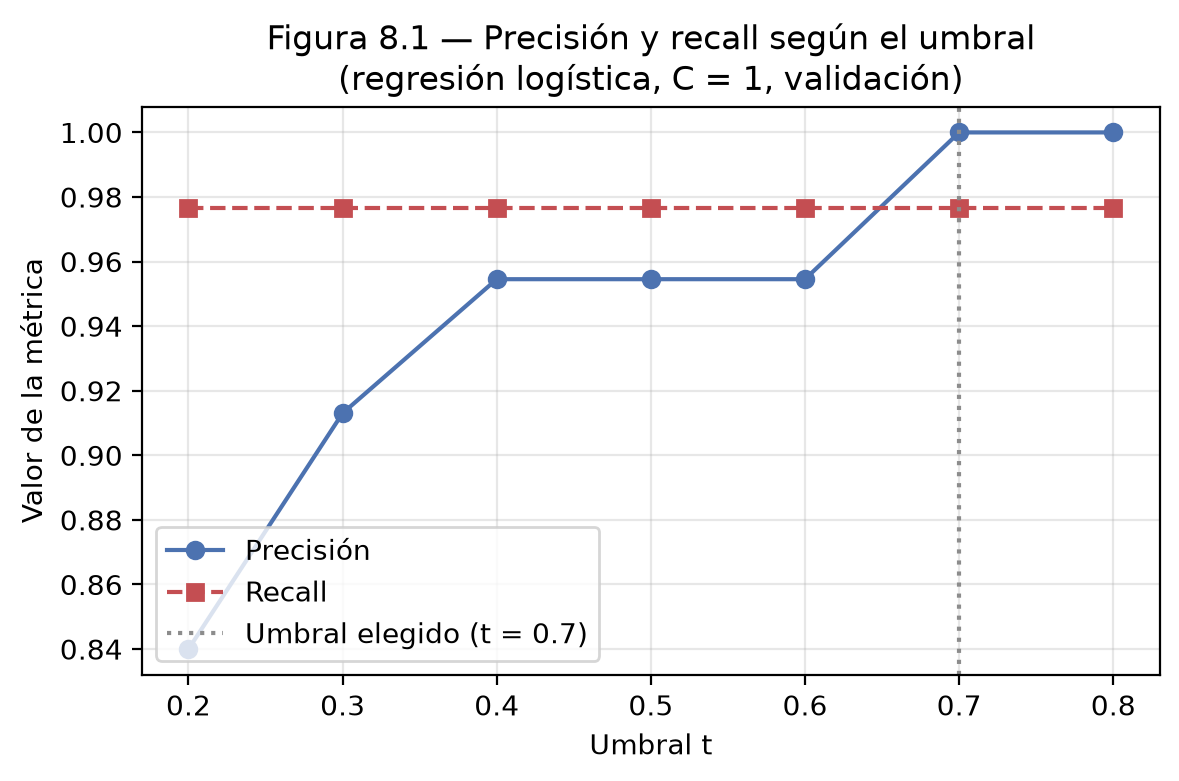
\includegraphics[width=0.68\textwidth]{figuras/ex8_precision_recall.png}
    \caption{Precisión y recall según el umbral, regresión logística con $C=\LogitC$ (validación).}
    \label{fig:ex8-pr}
\end{figure}

\item \textbf{Coeficientes estandarizados y odds.}
Recordemos del Ejercicio~3a que la regresión logística es lineal en los
log-odds: $\log\frac{p}{1-p}=\beta_0+\beta_1z_1+\dots+\beta_{30}z_{30}$, con
las $z$ estandarizadas. Así, cada coeficiente es lo que suben los
log-odds de malignidad cuando ese predictor aumenta una desviación
estándar de entrenamiento y los demás quedan fijos.

\begin{table}[H]
\centering
\small
% Archivo generado automáticamente por el notebook (no editar a mano).
\begin{tabular}{lrr}
\toprule
Predictor & Coeficiente & $e^{\beta}$ \\
\midrule
worst texture & 1.3553 & 3.8780 \\
mean concave points & 1.1043 & 3.0171 \\
radius error & 1.0259 & 2.7897 \\
worst symmetry & 0.9519 & 2.5905 \\
worst radius & 0.8134 & 2.2556 \\
worst area & 0.7948 & 2.2140 \\
area error & 0.7822 & 2.1864 \\
worst concavity & 0.7689 & 2.1575 \\
mean concavity & 0.7621 & 2.1428 \\
compactness error & $-$0.7591 & 0.4681 \\
\bottomrule
\end{tabular}

\caption{Diez mayores coeficientes estandarizados (en magnitud) de la regresión logística con $C=\LogitC$.}
\label{tab:ex8-coef}
\end{table}

Un coeficiente positivo indica que valores más altos del predictor se
asocian con mayor probabilidad de malignidad, y uno negativo lo contrario.
\texttt{worst texture} ($\CoefTexturaPeor$) y \texttt{mean concave points}
($\CoefPuntosConcavos$) salieron con signo positivo, coherente con que
núcleos de textura más irregular y con más hundimientos en el borde se
asocien con malignidad. En cambio \texttt{compactness error}
($\CoefCompactError$) salió con signo negativo, y nos tocó tener cuidado
al leerlo: no significa que valores altos de esa variable, por sí solos,
indiquen benignidad, sino que es un efecto condicional al resto de las 29
variables, muchas de ellas casi repetidas entre sí (radio, perímetro y área
miden casi lo mismo), y ya vimos en el Ejercicio~7 que en ese caso los
signos individuales pierden lectura.

Para pasar a odds se usa el factor $e^{\beta}$ del Ejercicio~3a. Para
\texttt{worst texture}, $e^{\CoefTexturaPeor}\approx\ExpTexturaPeor$: subir
una desviación estándar de entrenamiento multiplica los odds estimados de
malignidad por cerca de $\ExpTexturaPeor$, con las demás variables fijas.
Esto describe una asociación dentro del modelo y no un efecto causal. Con
esto dejamos congelados el pipeline con $C=\LogitC$ y el umbral
$t=\LogitT$.

\end{enumerate}
